\section{JHU Hydrodynamic Test Facility}
\label{appenJHUHTF.sec.hydrolab}
 
\begin{center}
\begin{figure}[t!]  
\subfigure[Johns Hopkins University Hydrodynamic Test Facility]
{  
    %
\includegraphics[trim=20cm 0mm 0mm 20cm,clip=true,width=80mm]{./appenJHUHTF/images/jhurov}
    \includegraphics[trim=0mm 10cm 0mm 25cm,clip=true,width=\textwidth]{./appenJHUHTF/images/hydroFacility}
}
\\
\subfigure[\ac{JHUROV} starboard side view]  
{
    \includegraphics[trim=0mm 20cm 0mm 125mm,clip=true,width=.56\textwidth]{./appenJHUHTF/images/jhurovStarboard}
    %\includegraphics[width=170mm]{./appenJHUHTF/images/hydroFacility}
}
\subfigure[\ac{JHUROV} stern view] 
{
    %\includegraphics[trim=20cm 0mm 0mm 20cm,clip=true,width=80mm]{./appenJHUHTF/images/jhurovStarboard}
    \includegraphics[trim=0mm 75mm 0mm 65mm,clip=true,width=.42\textwidth]{./appenJHUHTF/images/jhurovStern}
}
\caption{Johns Hopkins University Hydrodynamic Test Facility and \acf{JHUROV}.}
    \label{appenJHUHTF.fig.hydrolab}
\end{figure}
\end{center}


The Johns Hopkins Hydrodynamic Test Facility\cite{kinsey2003}
contains an indoor fresh water tank measuring \unit{7.75}{\m} in
diameter and \unit{4.25}{\m} deep, as shown in Figure
\ref{appenJHUHTF.fig.hydrolab}.  The facility is equipped with the
\ac{JHUROV}, a fully instrumented \ac{UV} designed for navigation and
control research.  The \ac{JHUROV} displaces \unit{150}{\kg} and is
actuated by six \unit{1.5}{\kWh} DC brushless electric direct drive
thrusters providing full control authority for 6-\ac{DOF}
maneuvers. Each thruster is controlled with a current-mode amplifier.
The \ac{JHUROV} control system generates the command current for each
thruster using data from {\it a-priori} {\it steady-state} thruster
calibration experiments; no feedback is used in generating the
commanded current.  The angular velocity of each thruster is
instrumented. This measured thruster angular velocity ($\omega_{th}$)
can be used to estimate the thruster force ($f_{th}$) using the
empirically validated steady state relation
$f_{th}=k_{th}\omega_{th}|\omega_{th}|$, where $k_{th}$ is an
empirically identified constant\cite{pona.book}.
%
The vehicle's control system is capable of actively controlling
6-\ac{DOF} vehicle motion.
%
During an experiment, each of the 6 \ac{JHUROV} \ac{DOF} were
independently actuated using either closed-loop control or open-loop
sinusoidal commanded torques. 
%
For the \acp{DOF} using closed-loop control,
a sinusoidal reference trajectory was specified to the \ac{JHUROV} control
system.



\begin{center}
\begin{figure}[htbp]
  \begin{center}
    \includegraphics[width=90mm]{./appenJHUHTF/images/refFrames}
  \end{center}
  \caption{ The world-frame's orthonormal x, y, and z basis vectors
    point from the frame's origin towards in the directions north,
    east, and down respectively. The body-frame's orthonormal x, y, and
    z basis vectors point from the vehicles origin to the vehicle's
    bow side, starboard side and keel location respectively. Note the
    arrows showing positive rotation about each body axis.}
  \label{appenJHUHTF.fig.refFrames}
\end{figure}
\end{center}


The coordinate frames employed herein are depicted in Figure
\ref{appenJHUHTF.fig.refFrames}.
%
The world-frame's orthonormal x, y, and z basis vectors point from the
frame's origin towards the direction north, east, and down
respectively.
%
Employing standard navel architecture conventions, the body-frame's
orthonormal x, y, and z basis vectors point, respectively, from the
vehicle's origin to the vehicle's bow, starboard side and keel.
%
The Euler angles heading, pitch, and roll express the relationship
between the world-frame and body-frame as follows: rotating the world-frame
about its +z-axis through an angle heading, then rotating the resulting
frame about its +y-axis through an angle pitch, then rotating the
resulting-frame around its +x-axis through an angle roll provides the
body-frame.


\begin{table}[htbp]
\ssp
\caption{\ac{JHUROV} state measurement sources, resolutions, and accuracies}
\begin{center}
\begin{tabular}{cccc}
% & & RefTraj1& RefTraj2 \\
%\hline
%\multicolumn{2}{c}{Reference Trajectory}  &Trajectory Control      &  Parameter \\
%\multicolumn{2}{c}{Purpose}              & Evaluation &  Cross-Validation \\
 & &  & Measurement \\
State & Source  & Update Rate &Precision/Std Dev  \\
& & &(Standard Deviation)\\
\hline\hline
XY Translational  & DVLNAV    & \unit{10}{\Hz} & Resolution $>$0.5\% of\\
Position & & &Translational Distance Traveled \\
\hline
Z Translational   & Digiquartz & \unit{7}{\Hz} & Resolution \\
Position & & & $>$0.75\% as calculated \\
\hline
Heading                 & PHINS III & \unit{10}{\Hz}& 0.13$^\circ$ Std Dev \\  
\hline
Pitch, Roll             & PHINS III & \unit{10}{\Hz}& 0.01$^\circ$ Std Dev \\  
\hline
Translational  & \unit{1200}{\kHz}  & \unit{6}{\Hz} & $>$0.003 m/s Std Dev \\  
Velocity & \acs{DVL}& & \\
\hline
Angular Velocity        & PHINS III & \unit{10}{\Hz}& 0.01$^\circ$/s Std Dev \\  
\hline \hline\end{tabular}
\end{center}
\label{appen_JHUHTF.tb.sensors}
%\vspace*{-5mm}
\end{table}


The sensors used in all experimental evaluations are recorded in Table
\ref{appen_JHUHTF.tb.sensors}.  
%
The \ac{JHUROV} is instrumented by a PHINS III \ac{INS} (IXSEA SAS,
Marly-le-Roi, France), \unit{1200}{\kHz} bottom-lock Doppler sonar (RD
Instruments, San Diego, CA), and 8CDP010-1 Digiquartz Depth Sensor
(Paroscientific Inc., Redmond, WA).  
%
The PHINS III \ac{INS} includes a three-axis north-seeking fiber-optic
gyrocompass, and inertial grade accelerometers whose data is used to
estimate angular velocity, pitch, roll, and heading states at a rate
of \unit{10}{\Hz}.  
%
For our PHINS configuration, the measurement error standard deviations
are 0.01$^\circ$/s for angular velocity estimates, 0.13$^\circ$ for
heading estimates, and 0.01$^\circ$ for pitch and roll
estimates\cite{PhinsManual2008}. The Doppler sonar measures the three
dimensional linear velocity in the instrument's frame with a standard
deviation of less than 0.003 m/s, an update rate of \unit{6}{\Hz}, and
zero bias\cite{NWHdataSheet}.
%
The Digiquartz has a maximum depth of 10 m and, as currently
configured, has an update rate of \unit{7}{\Hz}, and provides pressure
measurements at a resolution of 2 parts-per-million.
%
Translational position estimates are provided by the DVLNAV control
software which integrates the the sensor signals reported above to
provide dead reckoning XY translational position estimates better than
0.5\% of distance traveled.
%







